\chapter{Introduction}
\label{chapter_1}

During last decade, we have experienced a explosion in the growth of the social media, transforming the way we read the news, interact with our fiends and in general, how we consume content on the Internet. It has become in a tool used on a daily basis.

\begin{figure}[!htp]
  \center
  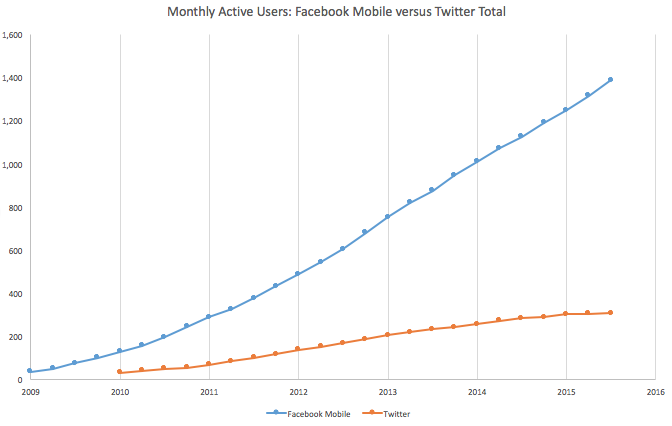
\includegraphics[width=0.75\textwidth]{figures/facebook_twitter_users.png}
  \caption{Evolution of social media: Facebook and Twitter active users in millions, image extracted from stratechery.}
  \label{fig:social media evolution}
\end{figure}

The growth of this kind of media, results on a vast amount of user generated content that are publicly available. The variety of the topic of the created content is very rich, as people tend to share comments about their hobbies, studies, work, relationships and, in general, daily live activities.

More and more researchers are using this media as a source from which conduct their experiments, as it eliminates the need to generate randomized data from the test phase of the experimentation and use a more reliable, real-life data. The ease with which data can be obtained along with the variety of content created in this media, has opened the door to new fields that would not be able to be researched. An example of this is \acrlong{sa}, the field of study that focuses on categorizing opinions and author's attitude towards a specific topic.

With the reduction of computational cost, has made possible the application of the before inviable mathematical models, improving both, the performance in these research field and and the popularity of these topics, resulting on the definition on new subtasks that derivate into the finding of new applications in which this researches could be used. To follow the previous example, emotion detection would be a \acrlong{sa} subtask that dives deeper on determine author's attitude towards a specific topic and aims to recognize the subject's emotional state.

Although previous work have been done in detecting irony or multiple emotions, such as happiness, sadness and fear, there is still little work that focuses just on anger and thus, the aim of this project is to study learn about the detection of anger, focusing on repressed anger, a topic that has multiple applications such as in helping in studies that focus on well being or customer reviews. At the same time, this project, serves to the author as a master's thesis and as an introduction to research and scientific world.

Throughout the following chapters, we will define that the term anger is and study how to detect repressed anger can be detected, answering to the question: \textit{``Can the repressed anger be detected in text?''}. We will then proceed with a review of the state of the art the fundamental on which this topic bases on, as a way to develop an accurate approach to solve this problem. Then, the results obtained by both, a naive approach and the proposed solution will be presented, compared and evaluated, ending up with the conclusion of this research and the future work still to be done.

\iffalse

\begin{itemize}
  \item Introduction
  \begin{itemize}
    \item Get the important points of the state of art referring to sentiment analysis, repressed anger detection.
    \item Explain the hypothesis to be worked out in the thesis.
  \end{itemize}

  \item Planning and Methodology [OK]
  \begin{itemize}
    \item Explain the plan. [OK]
    \item Explain the methodology. [OK]
    \item Show the schedule. [OK]
  \end{itemize}

  \item State of art
  \begin{itemize}
    \item Explain that sentiment analysis is.
    \item Explain what emotion analysis is, compared to previous point.
    \item Explain previous work.
    \begin{itemize}
      \item Previous work in anger detection.
      \item Previous work in irony detection.
    \end{itemize}
    \item Explain the that the project will focus on resolve the issue as a text classification problem.
    \begin{itemize}
      \item Classification Techniques 
      \item Fundamentals of Classification 
      \item General classification problem solving
      \item Explain the algorithms I used to make tests in WEKA.
      \item Explain Deep Learning.
      \begin{itemize}
        \item Explain Convolutional neural networks.
      \end{itemize}
    \end{itemize}
  \end{itemize} 

  \item Development
  \begin{itemize}
    \item Early development on the exploration phase.
    \begin{itemize}
      \item WEKA text classification testing.
    \end{itemize}
    \item Explain that on SemEval they said that the best scoring system were using DL and is becoming trending. General Problem Solving techniques (NPL) in Deep Leaning perform better that those that focus on resolving in depth focusing on the topic.
    \begin{itemize}
      \item Change to Deep Learning Development.
      \item Explain the usage of architecture that Yoon Kim uses. (Previously explained in SoA)
      \item Explain the process to detect repressed anger. (The system I made starting from dataset merging, ending with merge of 2 classification output.) Simple diagram.
      \begin{itemize}
        \item Dataset searching and generation.

          --> Developed a tweet downloader for IDs.

        \item Word2vec (needed for CNN)

          --> Model used for Word2vec.
          
          --> Spell checking
          
          --> Slang dictionaries (difficulty on when to process the word. Detect Slang)
          
          --> Usage of Stopwords.

        \item CNN classifiers

          --> hyperparams used.

        \item Classification output merge.
        
        --> Due to the labels in the dataset cannot use ensemble learning and use a 2x2 matrix to match everything.
        
        --> Develop a automatic Google forms and how to process them back to the original dataset.
      \end{itemize}
    \end{itemize}
  \end{itemize}

  \item Research Framework
  \begin{itemize}
    \item Searching datasets, or create one, automatically.
    \item Manual labeling used to final prediction process.
  \end{itemize}

  \item Results
  \begin{itemize}
    \item Google Model
    \begin{itemize}
      \item Explain the final result plus each classification independently.
    \end{itemize}
    \item Twitter Model
    \begin{itemize}
      \item Explain the final result plus each classification independently. 
    \end{itemize}
    \item Spell checking
  \end{itemize}

  \item Conclusion and Future Work
    \begin{itemize}
      \item Different approach now that manual label data is obtained.  (Semi-supervised learning) 
    \end{itemize}
  
  \item Self-assessment
  \begin{itemize}
    \item writing.
  \end{itemize}
\end{itemize}

\fi
